\documentclass[tikz]{standalone}
\usepackage[sfdefault,light]{roboto}
\usetikzlibrary{
	arrows,
	arrows.meta,
	chains,
	positioning,
	shapes,
	shapes.multipart,
	mindmap,
	fit,
	calc,
	intersections,
	backgrounds,
	scopes,
	matrix,
	shadows,
}
\tikzset{every picture/.style={/utils/exec={\sffamily}}}
\definecolor{MyGreen}{HTML}{41B3A3}
\definecolor{MyOrange}{HTML}{f0884e}
\newcommand{\alert}[1]{{\color{MyOrange} #1}}
\begin{document}
    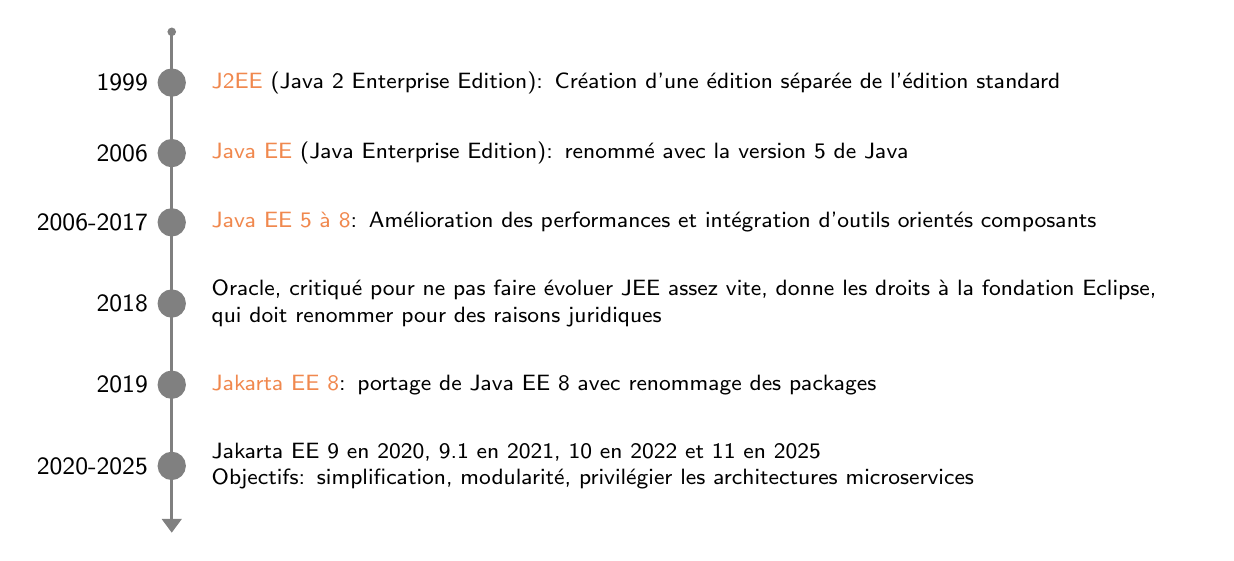
\begin{tikzpicture}[
        every node/.style={font=\small},
		node distance = 1mm and 3mm,
		start chain = A going below,
		dot/.style = {circle, draw=gray, thick, fill=gray,
			minimum size=2mm},
		box/.style = {rectangle, text width=\textwidth,
			inner xsep=5mm, inner ysep=2.5mm,
			font=\sffamily\footnotesize,%\linespread{0.84}\selectfont,
			on chain},
	]
	\begin{scope}[every node/.append style={box}]
		\node { \alert{J2EE} (Java 2 Enterprise Edition): Création d'une édition séparée de l'édition standard } ;
		\node { \alert{Java EE} (Java Enterprise Edition): renommé avec la version 5 de Java} ;
		\node { \alert{Java EE 5 à 8}: Amélioration des performances et intégration d'outils orientés composants} ;
		\node { Oracle, critiqué pour ne pas faire évoluer JEE assez vite, donne les droits à la fondation Eclipse, qui doit renommer pour des raisons juridiques} ;
		\node { \alert{Jakarta EE 8}: portage de Java EE 8 avec renommage des packages } ;
		\node { Jakarta EE 9 en 2020, 9.1 en 2021, 10 en 2022 et 11 en 2025 \\
            Objectifs: simplification, modularité, privilégier les architectures microservices} ;
	\end{scope}
	\draw[	
		very thick, gray, 
		{Circle[length=3pt]}-{Triangle[length=5pt)]},
		shorten <=-3mm, shorten >=-3mm
	]           % <--- here is adjusted additional arrow's 
	(A-1.north west) -- (A-6.south west);
	\foreach \i [ count=\j] in {1999,2006,2006-2017,2018,2019,2020-2025}
		\node[dot,label=left:\i] at (A-\j.west) {};
	\end{tikzpicture}
\end{document}